\chapter{Evaluation}
\label{cha:evaluation}

\section{Bewertung der Datenqualität und -validität}
\begin{spacing}{1.5}

Insgesamt wurden 5.000 synthetische Daten generiert. \acrshort{sdv} verfügt über eingebaute Funktionen zur Bewertung der synthetischen Daten und zur Gewinnung weiterer Erkenntnisse. Die \acrshort{sdv}-Diagnose führt einige grundlegende Validitätsprüfungen\footnote{\url{https://docs.sdv.dev/sdv/single-table-data/evaluation/diagnostic\#whats-included}} durch:

\begin{itemize}
  \item Alle Primärschlüssel müssen eindeutig sein.
  \item Stetige Werte müssen mit den Minimal- und Maximalwerten der realen Daten übereinstimmen.
  \item Diskrete Spalten müssen die gleichen Kategorien haben wie die echten Daten.
\end{itemize}

Die \acrshort{sdv}-Diagnose ergab, dass die generierten Daten zu 100 \% valide sind. Eine daraufhin ausgeführte Auswertung der Datenqualität (evaluate\_quality) ergab, dass die synthetischen Daten zu 86,1 \% mit den realen Daten hinsichtlich ihrer statistischen Eigenschaften (z. B. Korrelation \& Randverteilung) übereinstimmen. Eine detaillierte Aufschlüsselung der Korrelationswerte kann Tabelle \ref{tab:correlation-detailled} entnommen werden.

\newpage

\begin{table}[!htb]
    \centering\footnotesize
    \begin{tabular}{lll}
        \toprule
        \\[-0.7em]
        Attribut & Datentyp & Korrelation [\%] \\
        \\[-0.9em]
        \midrule
        \\[-0.7em]
        income & kategorisch & 0.982810 \\
        age & nummerisch & 0.956845 \\
        sex & kategorisch & 0.945395 \\
        dob & datetime & 0.947869 \\
        education-num & nummerisch & 0.952392 \\
        workclass & kategorisch & 0.933288 \\
        hours-per-week & nummerisch & 0.927463 \\
        education & kategorisch & 0.924603 \\
        marital-status & kategorisch & 0.904812 \\
        race & kategorisch & 0.901783 \\
        relationship & kategorisch & 0.872116 \\
        fnlwgt & nummerisch & 0.865818 \\
        pob & kategorisch & 0.808084 \\
        capital-loss & nummerisch & 0.800251 \\
        native-country & kategorisch & 0.799960 \\
        occupation & kategorisch & 0.770835 \\
        capital-gain & nummerisch & 0.689690 \\
        \\[-0.9em]
        \bottomrule
    \end{tabular}
    \caption[Detaillierte Korrelationswerte der synthetischen Daten]{Detaillierte Korrelationswerte der synthetischen Daten\footnotemark}
    \label{tab:correlation-detailled}
\end{table}
\footnotetext{Eigene Darstellung}

\end{spacing}
\section{Vergleichende Analyse mit realen Daten}
\label{sec:comparing-analysis}
\begin{spacing}{1.5}

Vergleicht man die generierten synthetischen Daten mit den realen Daten, so fällt zunächst auf, dass diese auf den ersten Blick nicht voneinander unterscheidbar sind -- abgesehen von der Reihenfolge der Spalten (vgl. Anhang 1). Im ursprünglichen Datensatz war mit der Adresse auch ein sensitives (wenn auch fiktives) Attribut enthalten. Dieses wurde durch den Synthesizer automatisch erkannt und vollkommen anonymisiert, indem mithilfe der Python-Bibliothek \textit{Faker} grundlegend neue, gefälschte Werte erstellt werden, die lediglich der Syntax des Originals entsprechen.

Eine detaillierte Betrachtung der Datenqualität erfolgt anhand mehrerer Vergleichsdiagramme. Abbildung \ref{fig:real-vs-synthetic-age} zeigt die Altersverteilungen in den realen und synthetischen Datensätzen. Man erkennt, dass die allgemeine Form der Verteilung in beiden Datensätzen sehr ähnlich ist, was darauf hinweist, dass der Synthesizer die Altersstruktur der Bevölkerung gut reproduziert hat.  Auffällig ist, dass die synthetischen Daten eine höhere relative Häufigkeit in der Altersgruppe von etwa 35 Jahren aufweisen und zwei weitere Hochpunkte bei etwa 22 und 46 Jahren zeigen. Im Vergleich dazu sind die realen Daten gleichmäßiger verteilt. Diese Auffälligkeit kann auf den Synthesizer selbst zurückgeführt werden, welcher dazu neigt, bestimmte Muster zu glätten, zu extrapolieren oder mit Rauschen zu überlagern\footnote{\url{https://docs.sdv.dev/sdv/multi-table-data/evaluation/data-quality\#interpreting-the-score}}.

\begin{figure}[ht]
\begin{center}
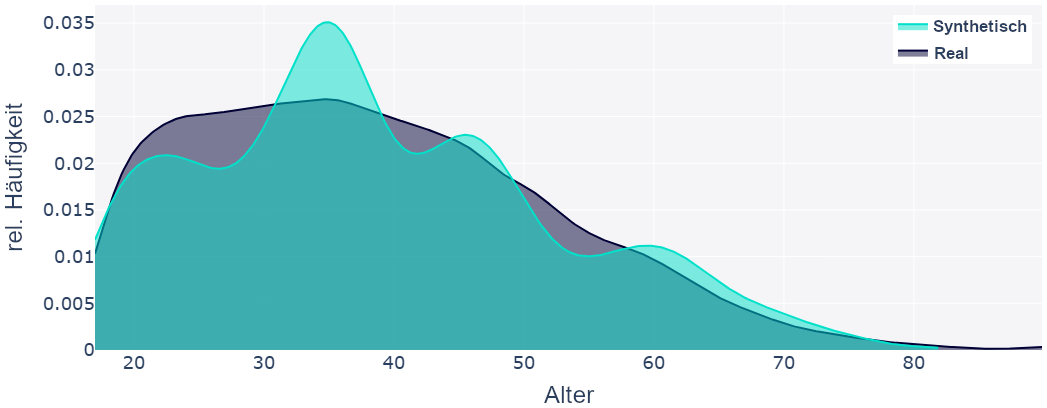
\includegraphics[width=\textwidth]{img/real-vs-synthetic-age.png}
\caption[Verteilung des Attributs \textit{age} in realen und synthetischen Daten]{Verteilung des Attributs \textit{age} in realen und synthetischen Daten}
\label{fig:real-vs-synthetic-age}
\end{center}
\end{figure}

\begin{figure}[ht]
\begin{center}
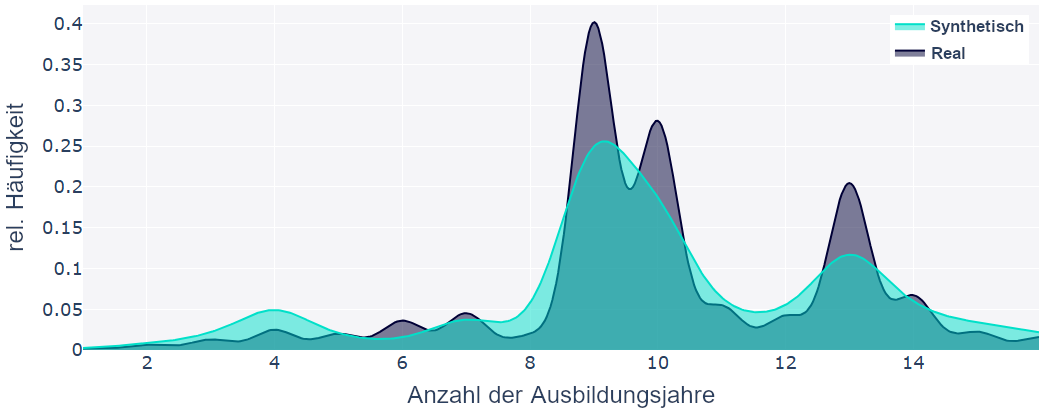
\includegraphics[width=\textwidth]{img/real-vs-synthetic-education.png}
\caption[Verteilung des Attributs \textit{education-num} in realen und synthetischen Daten]{Verteilung des Attributs \textit{education-num} in realen und synthetischen Daten}
\label{fig:real-vs-synthetic-education}
\end{center}
\end{figure}

Ein ähnliches Phänomen ist in Abbildung \ref{fig:real-vs-synthetic-education} zu beobachten. Im Gegensatz zur Verteilung des Alters zeigt die Verteilung des Attributs \textit{education-num} in den synthetischen Daten jedoch eine deutlich glattere Kurve. Dies deutet darauf hin, dass der Synthesizer hier eine stärkere Glättung vorgenommen hat, um die Verteilung der Bildungsniveaus nachzubilden. Während die reale Datenverteilung kleine Schwankungen und Unregelmäßigkeiten aufweist, sind diese in den synthetischen Daten weitgehend geglättet worden. Dies kann dazu führen, dass bestimmte Feinheiten der realen Daten nicht vollständig in den synthetischen Daten widergespiegelt werden, was bei der Interpretation und Verwendung der synthetischen Daten berücksichtigt werden muss.

\begin{figure}[ht]
\begin{center}
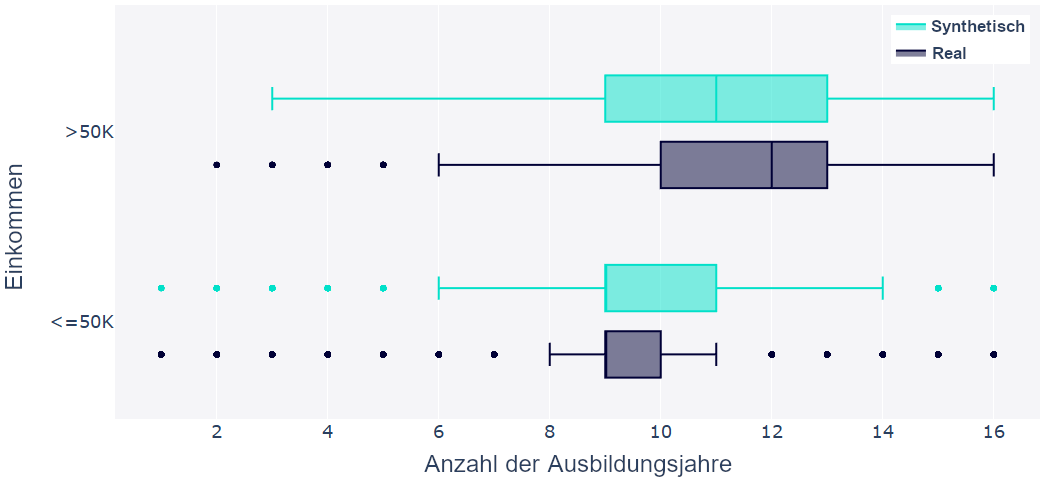
\includegraphics[width=\textwidth]{img/income-vs-education.png}
\caption[Attribut \textit{income} in Abhängigkeit zum Attribut \textit{education-num}]{Attribut \textit{income} in Abhängigkeit zum Attribut \textit{education-num}}
\label{fig:income-vs-education}
\end{center}
\end{figure}

Abbildung \ref{fig:income-vs-education} zeigt mehrere Box-Plots und visualisiert die Korrelation zwischen Bildung und Einkommen sowohl in den realen als auch in den synthetischen Daten. Die synthetischen Daten reproduzieren die positive Korrelation zwischen höheren Bildungsabschlüssen und höherem Einkommen, die auch in den realen Daten zu beobachten ist. Anhand der Box-Plots fällt jedoch auf, dass die Streuung in den synthetischen Daten größer ist.

\end{spacing}